\section{Linear-Size Additive Spanners in Sub-quadratic Time}
\label{sec: subq}

In this section we provide the proof of \Cref{subquad}. 
We will first show in \Cref{sec: subquad for 3/7} a simple subquadratic time algorithm for computing an $\tilde O(n^{3/7+\eps})$ additive spanner.
Then we will slightly modify it to achieve better additive error bound in \Cref{sec: proof of subquad}.

\subsection{A subquadratic time algorithm for $\tilde O(n^{3/7+\eps})$ additive spanner}
\label{sec: subquad for 3/7}

In this subsection, we prove the following theorem, which shows that an additive spanner with the current best error (as in \cite{bodwin2021better}) can be computed in subquadratic time.

\begin{theorem}\label{subquad for 3/7}
There is an algorithm, that, given any undirected unweighted graph on $n$ vertices and $m$ edges, and any parameter $\eps > 0$, computes a spanner on $O\brac{2^{O(1/\eps)}\cdot n\log n}$ edges with $\tilde O(n^{3/7+\eps})$ additive stretch, in time $\tilde{O}\big(m + 2^{O(1/\eps)}\cdot n^{13/7}\big)$.
\end{theorem}
\begin{remark}
	If we do not care about the runtime constraint, then the spanner size can be made $2^{O(1/\epsilon)}n$ by replacing \Cref{clustering} with the original Lemma 13 from \cite{bodwin2021better}.
\end{remark}

We start with the following lemma for a preliminary sparsification of the input graph.
%Since we are aiming for $\tilde{O}(n^{3/7+\epsilon})$ additive stretch, the following lemma says that we can safely assume $G$ is a sparse graph.
\begin{lemma}\label{preproc}
There is an algorithm, that given any graph $G$ and parameter $1<d<n$, computes in $\tilde{O}(m)$ time an $+\tilde O(n/d)$ spanner $G'$ of $G$ with $|E(G')|\le O(nd)$ edges.
%such that for any $s, t\in V$, we have $\dist_{G^\prime}(s, t)\leq \dist_G(s, t) + \tilde{O}(n/d)$; plus, $G^\prime$ can be constructed 
\end{lemma}
\begin{proof}
Graph $G^\prime$ is simply the union of (i) for each vertex $v\in V(G)$ with $\deg_G(v) \leq \ceil{d}$, all incident edges of $v$; and (ii) an $O(\log n)$-multiplicative spanner of $G$ with $O(n)$ edges; such a multiplicative spanner can be computed in $\tilde{O}(m)$ time as shown in \cite{baswana2007simple}. Clearly, graph $G'$ can be computed in $\tilde O(m)$ time.
	
Consider now any pair $s, t\in V(G)$ and let $\pi$ be an $s$-$t$ shortest path in $G$. 
It is easy to observe that at most $O(n/d)$ vertices in $\pi$ have degree more than $d$, so the number of edges in $E(\pi)$ that is incident to any degree $\le d$ vertex is at most $O(n/d)$. As we have included in $G'$ an $O(\log n)$-multiplicative spanner of $G$, the distance in $G'$ between the pair of endpoints of every such edge is at most $O(\log n)$.
Therefore, $\dist_{G'}(s,t)\le \dist_G(s,t)+\tilde{O}(n/d)$.
\end{proof}

We now proceed to describe our algorithm for \Cref{lem: reduction}. Similar to \Cref{sec: subset}, we assume that the (unit) edge weights are slightly perturbed so that for every pair $s,t$ there is a unique shortest path connecting them in $G$ (or any subgraph that contains both $s$ and $t$).

As a pre-processing step, if $|E(G)|\ge 10\cdot n^{2-3/7}$, then we first apply the algorithm from \Cref{preproc} to $G$ with $d=n^{1-3/7}$,
%By the above lemma, choosing $d = \ceil{n^{3/7}}$, for the rest we reduce to the case where $G$ itself has at most $O(n^{11/7})$ edges by a $\tilde{O}(m)$ runtime overhead.
and get graph $G'$, so $|E(G')|=O(n^{2-3/7})$.
If $|E(G)|\le 10\cdot n^{2-3/7}$, then we simply set $G'=G$.

%Without loss of generality, Note that we can assume that $G$ is connected, as otherwise we simply focus on different connected components of $G$, so $$.  
%The main algorithm utilizes the power of Lemma \ref{clustering}. 
We then apply the algorithm from \Cref{clustering} to $G'$ with parameter $R$ (to be determined later) and $\frac{10}{\epsilon\log_2n}$, and let $\bset$ be the set of balls we obtain.
%
\iffalse
each radius $r = [R, Rn^\epsilon]$ in $\tilde{O}(2^{10/\epsilon}m)$ time with two properties:
 \begin{itemize}
	\item (Coverage) For each $v\in V$, there is some ball such that $v\in \ball_G(c, r)\in \bset$.
	\item (Disjointness) $\sum_{\ball(c, r)\in\bset}|\ball(c, 4r)| = \tilde{O}(2^{10/\epsilon}n)$, $\sum_{\ball(c, r)\in\bset}\vol(\ball(c, 4r)) = \tilde{O}(2^{10/\epsilon}m)$.
\end{itemize}

For any ball $\ball(c, r)\in\bset$, classify it as one of the following two types.
\begin{itemize}
	\item (Small) $|\ball(c, r)| \leq R^{5/3}$.
	\item (Large) $|\ball(c, r)| > R^{5/3}$.
\end{itemize}
\fi 
We say that a ball $\ball(c, r)\in\bset$ is \emph{small} if $|\ball(c, r)| \leq R^{5/3}$; otherwise we say it is \emph{large}.
For each ball $\ball(c,r)\in \balls$, we compute a BFS tree $T_c$ that is rooted at $c$ and spans all vertices in $\ball(c, 4r)$, in time $O(\vol(\ball(c, 4r)))$. From \Cref{clustering}, $\sum_{c} |E(T_c)|= \sum_{c} |\ball(c, 4r)| = O(2^{10/\epsilon}n\log n)$.



%For the rest we will mainly work on the sparse graph $G$. Let $H$ denote the target additive spanner of $G$. $H$ is constructed from an empty graph. First, for each ball $\ball(c, r)\in \bset$, add an arbitrary breath-first search tree at $c$ that spans $\ball(c, 4r)$ to $H$. Next, add two different types of subset spanners to $H$.
%\vspace{-10pt}

\paragraph{Handling small balls.} Consider a small ball $\ball(c, r)\in \bset$. From Lemma \ref{bottleneck}, we can compute in time $O(\vol(\ball(c, 4r)))$ an integer $d\in [r, 2r]$ such that $|\ball^=(c, d)\cup\ball^=(c, d+1)|\leq 2|\ball(c, 4r)| / r \leq 2|\ball(c, 4r)| / R$. We denote  %For notational convenience, denote: 
$\bset_1 = \{\ball(c, d)\mid \ball(c, r)\in\bset\text{ is small} \}$.
%Next, we will build a distance preserver $X_c\subseteq G[\ball(c, 4r)]$ such that $\dist_{X_c}(s, t) = \dist_{G}(s, t)$ for any pair $s, t\in \ball^=(c, d)\cup\ball^=(c, d+1)$. To do this, go over each vertex $s\in \ball^=(c, d)$ and compute single-source shortest paths at $s$ in $G[\ball(c, 4r)]$. By doing so, we can collect a set $\Pi_c = \{\pi_{s, t} \mid s, t\in \ball(c, d)\cup\ball(c, d+1) \}$ of shortest paths between any pair of vertices in $\ball(c, d)\cup\ball(c, d+1)$; we can make sure that $\paths$ is consistent by randomly perturbing the unit edge weights of $G[\ball(c, 4r)]$. 
%We then apply the algorithm from \Cref{cor: BFS consistent} to the induced subgraph $G[\ball(c, 4r)]$ with $S=T=\ball^=(c, d)\cup\ball^=(c, d+1)$, and obtain a collection $\Pi_c$ of shortest paths. We define $R_c=\bigcup_{\pi\in \Pi_c}\pi$.
%Add all edges in $\bigcup_{c, \pi\in \Pi_c}\pi$ to $X$. According to Lemma \ref{consist}, each path system $\Pi_c$ contains edges at most 
%From \Cref{cor: BFS consistent} and \Cref{clustering}, $$\sum_{c} |E(R_c)|= \sum_{c} O\left(|\ball(c, 4r)| + \sqrt{|\ball(c, 4r)|}\cdot \left(\frac{|\ball(c, 4r)|}{R}\right)^2\right) = \sum_c O(2^{15/\epsilon}|\ball(c, 4r)|)=O(2^{25/\epsilon}n/\eps)$$
\iffalse
\paragraph{Local subset spanner.} For each small ball $\ball(c, r)\in \bset$, apply Lemma \ref{bottleneck} to find a radius $d\in [r, 2r]$ such that $|\ball^=(c, d)\cup\ball^=(c, d+1)|\leq 2|\ball(c, 4r)| / r$; also when $\ball(c, r)$ is large, simply set $d = r$. For notational convenience, define 
$$\bset_1= \{\ball(c, d)\mid \ball(c, r)\in\bset\}$$
\fi
Then, for each small ball $\ball(c, r)$, apply Lemma \ref{subset} to compute a subset spanner $L_c$ of $G'[\ball(c, 4r)]$ on the set $\ball^=(c, d)\cup\ball^=(c, d+1)$.

%\paragraph{Global subset spanner.} Sample a random vertex subset $S$ of size $\ceil{10R^{2/3}\log n}$ from the multi-set $$\biguplus_{\ball(c, r)\in \bset}\ball(c, 4r)$$ 

%\vspace{-10pt}

\paragraph{Handling large balls.}
Choose a random subset $S\subseteq V(G)$ of size $\ceil{10R^{2/3}\log n}$.
% from the multi-set $\biguplus_{\ball(c, r)\in \bset}\ball(c, 4r)$.
We then apply Lemma \ref{subset} to compute a subset spanner $\hat H$ of $G'$ on $S$.

\paragraph{The spanner construction.}
The output graph $H$ is simply defined to be the union of 
\begin{itemize}
	\item for each ball $\ball(c,r)\in \balls$, the tree $T_c$;
	\item for each small ball $\ball(c,r)\in \balls$, graph $L_c$;
	\item graph $\hat H$.
\end{itemize}


\subsubsection{Stretch analysis}

According to \Cref{preproc}, in order to show that $H$ is a $+\tilde O(n^{3/7+\eps})$ spanner of $G$, it suffices to show that $H$ is a $+\tilde O(n^{3/7+\eps})$ spanner of $G'$. For notational convenience, in this subsection we rename $G'$ by $G$.
%
The following statement, which is a generalization of \Cref{exact}, is the key to the stretch analysis.
\begin{claim}\label{exact2}
Let $s,t$ be a pair of vertices in $G$ and let $\pi$ be a shortest path connecting them. Then there exists (i) a path $\phi$ in $H$ connecting $s$ to $t$; (ii) a sequence of balls $\ball(c_1, r_{1}), \ldots, \ball(c_l, r_{l})$; (iii) two sequences of vertices $(u_0 = s, u_1, \ldots, u_l = t)$ and $(v_0 = s, v_1, \ldots, v_{l-1})$, and two sequences of paths  $\alpha_1, \alpha_2, \ldots, \alpha_l$, $\beta_1, \beta_2, \ldots, \beta_l$, with the following properties.
	\begin{enumerate}[(a),leftmargin=*]
		\item Vertices $u_1, u_2, \ldots, u_l$ appear on path $\pi$ in this order in the direction from $s$ to $t$.
		\item $s\in \ball(c_1, d_{1}), t\in\ball(c_l, d_{l}+1)$, and $v_i\in \ball^=(c_{i+1}, d_{{i+1}}), u_i\in \ball^=(c_i, d_{i}+1), \forall 1\leq i\leq l-1$.
		\item For each $1\leq i\leq l$, $\alpha_i$ is a shortest path in $H$ connecting $v_{i-1}$ to $u_i$ that is entirely contained in $G[\ball(c_i, 4r_{i})]$, and moreover, vertex $v_i$ lies on $\alpha_i$.
		\item For each $1\leq i\leq l-1$, $\beta_i = \alpha_i[v_{i-1}, v_i]$; and $\beta_l = \alpha_l$.
		\item $\phi=\beta_1\circ \cdots \circ \beta_l$; and $|\phi|\leq \dist_{G}(s, t) + 15\cdot Rn^\epsilon + \tilde{O}\left(2^{15/\epsilon}\cdot n^\epsilon\cdot\sum_{i=2}^{l-1}\frac{|\ball(c_i, r_{i})|}{R^{2/3}}\right)$.
	\end{enumerate}
\end{claim}

\begin{figure}[h]
	\begin{center}
		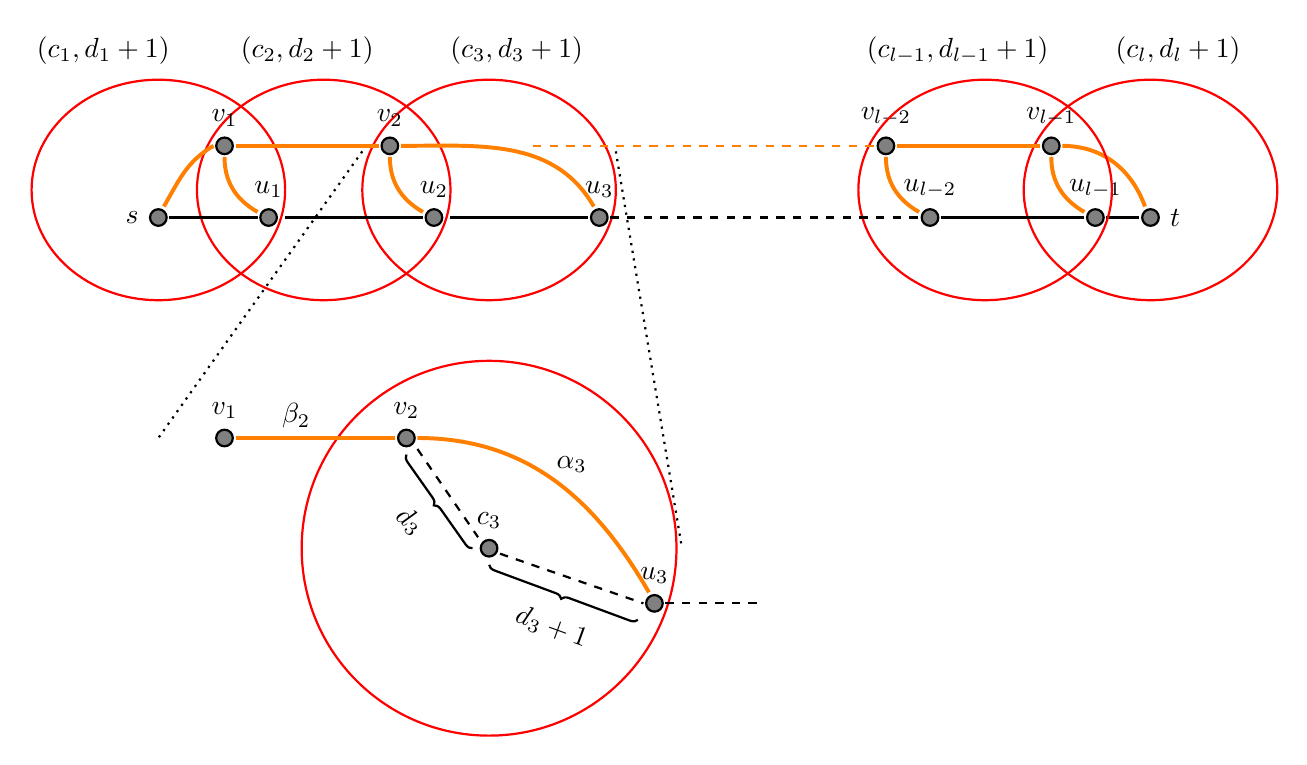
\begin{tikzpicture}[thick,scale=0.7]
	\draw [red] (0, 0.5) ellipse (2.3 and 2);
	\draw [red] (3, 0.5) ellipse (2.3 and 2);
	\draw [red] (6, 0.5) ellipse (2.3 and 2);
	\draw [red] (18, 0.5) ellipse (2.3 and 2);
	
	\draw (0, 0) node[circle, draw, fill=black!50, inner sep=0pt, minimum width=6pt, label = 180 : $s$] {};
	\draw (18, 0) node[circle, draw, fill=black!50, inner sep=0pt, minimum width=6pt,label = 0 : $t$] {};
	
	\draw (2, 0) node[circle, draw, fill=black!50, inner sep=0pt, minimum width=6pt,label = $u_1$] {};
	\draw (1.2, 1.3) node[circle, draw, fill=black!50, inner sep=0pt, minimum width=6pt,label = $v_1$] {};
	\draw [line width = 0.5mm] (0.2, 0) -- (1.8, 0);
	\draw [line width = 0.5mm, color=orange] (0.1, 0.2) to[out=60, in=210] (1, 1.3);
	\draw [line width = 0.5mm, color=orange] (1.2, 1.1) to[out=-90, in=150] (1.8, 0.1);
	
	\draw (-1, 2.4) node[red, label={$\ball(c_1, d_{1}+1)$}]{};
	
	\draw (5, 0) node[circle, draw, fill=black!50, inner sep=0pt, minimum width=6pt,label = $u_2$] {};
	\draw [line width = 0.5mm] (2.3, 0) -- (4.8, 0);
	
	\draw (2.7, 2.4) node[red, label={$\ball(c_2, d_{2}+1)$}]{};
	\draw [line width = 0.5mm, color=orange] (1.4, 1.3) -- (4, 1.3);
	\draw [line width = 0.5mm, color=orange] (4.2, 1.1) to[out=-90, in=150] (4.8, 0.1);
	
	\draw (4.2, 1.3) node[circle, draw, fill=black!50, inner sep=0pt, minimum width=6pt,label = $v_2$] {};
	\draw (8, 0) node[circle, draw, fill=black!50, inner sep=0pt, minimum width=6pt,label = $u_3$] {};
	\draw [line width = 0.5mm] (5.3, 0) -- (7.8, 0);
	
	\draw (6.5, 2.4) node[red, label={$\ball(c_3, d_{3}+1)$}]{};
	\draw [line width = 0.5mm, color=orange] (4.4, 1.3) to[out=0, in=120] (7.9, 0.2);
	
	\draw[dotted] (3.7, 1.2) -- (0, -4);
	\draw[dotted] (8.3, 1.2) -- (9.5, -6);
	\draw (4.5, -4) node[circle, draw, fill=black!50, inner sep=0pt, minimum width=6pt,label = $v_2$] {};
	\draw (9, -7) node[circle, draw, fill=black!50, inner sep=0pt, minimum width=6pt,label = $u_3$] {};
	\draw (6, -6) node[circle, draw, fill=black!50, inner sep=0pt, minimum width=6pt,label = $c_3$] {};
	\draw [red] (6, -6) ellipse (3.4 and 3.4);
	%\draw [dashed] (2, -7) -- (8.8, -7);	
	\draw [dashed] (9.2, -7) -- (11, -7);
	\draw [line width = 0.5mm, color=orange] (4.7, -4) to[out=0, in=120] (8.9, -6.8);
	\draw (7.5, -5) node[red, label={$\alpha_3$}]{};
	\draw [line width = 0.5mm, color=orange] (1.4, -4) to (4.3, -4);
	\draw (1.2, -4) node[circle, draw, fill=black!50, inner sep=0pt, minimum width=6pt,label = $v_1$] {};
	\draw (2.5, -4.2) node[red, label={$\beta_2$}]{};
	
	\draw [decorate, decoration = {brace}] (5.7,-6) -- (4.5,-4.3);
	\draw [dashed] (4.7, -4.2) -- (5.8, -5.8);
	\draw (4.3, -6) node[label={[rotate=-40]$d_3$}]{};
	\draw [decorate, decoration = {brace}] (8.7, -7.3) -- (6, -6.3);
	\draw [dashed] (6.2, -6.1) -- (8.8, -7);
	\draw (7, -8) node[label={[rotate=-20]$d_3+1$}]{};
	
	\draw (16.2, 1.3) node[circle, draw, fill=black!50, inner sep=0pt, minimum width=6pt,label = $v_{l-1}$] {};
	\draw (17, 0) node[circle, draw, fill=black!50, inner sep=0pt, minimum width=6pt,label = $u_{l-1}$] {};
	\draw [line width = 0.5mm] (17.8, 0) -- (17.2, 0);
	
	\draw [line width = 0.5mm, color=orange] (16.4, 1.3) to[out=0, in=110] (17.9, 0.2);
	
	\draw (18.5, 2.4) node[red, label={$\ball(c_l, d_{l}+1)$}]{};
	
	\draw (13.2, 1.3) node[circle, draw, fill=black!50, inner sep=0pt, minimum width=6pt,label = $v_{l-2}$] {};
	\draw (14, 0) node[circle, draw, fill=black!50, inner sep=0pt, minimum width=6pt,label = $u_{l-2}$] {};
	\draw [line width = 0.5mm] (16.8, 0) -- (14.2, 0);
	\draw [red] (15, 0.5) ellipse (2.3 and 2);
	\draw (14.5, 2.4) node[red, label={$\ball(c_{l-1}, d_{l-1}+1)$}]{};
	\draw [line width = 0.5mm, color=orange] (13.2, 1.1) to[out=-90, in=150] (13.8, 0.1);
	\draw [line width = 0.5mm, color=orange] (13.4, 1.3) -- (16, 1.3);
	\draw [line width = 0.5mm, color=orange] (16.2, 1.1) to[out=-90, in=150] (16.8, 0.1);
	
	\draw [dashed, color=orange] (6.8, 1.3) -- (13.1, 1.3);
	\draw [dashed] (8.2, 0) -- (13.8, 0);
\end{tikzpicture}
		\caption{The construction of vertex sequences $u_1, u_2, \ldots, u_l$ and $v_1, v_2, \ldots, v_{l-1}$; the orange paths belong to the spanner $H$.}\label{add-err}
	\end{center}
\end{figure}

\begin{proof}
%Let us determine $\phi$ and all the auxiliary structures by an iterative procedure that scans $\pi$ from $s$ to $t$. The iterative procedure perform the following steps. See Figure \ref{add-err} for an illustration.
Start with $i=0$. Before iteration $i$, suppose we have already computed vertices $u_1, u_2, \ldots, u_i$, and $v_1, v_2, \ldots, v_{i-1}$, and paths $\alpha_1, \alpha_2, \ldots, \alpha_i$, and paths $\beta_1, \beta_2, \ldots, \beta_{i-1}$. During the algorithm, keep $\phi = \beta_1\circ \beta_2\cdots\circ \beta_{i-1}\circ\alpha_i$. So $\phi$ is a path in $H$ from $s$ to $u_i$.

\begin{enumerate}[(1),leftmargin=*]
	\item If $u_i = t$ then we terminate the process and let $l=i$.
	
	Otherwise, find the ball  in $\bset_1$ that, among all balls in $\bset_1$ that intersects with $\phi$, the one that contains a vertex on $\pi$ that is closest to $t$. Note that this ball always exists; for example we can pick an arbitrary one that contains $u_i$.
	
	We denote this ball by $\ball(c_{i+1}, d_{i+1})$ and set $u_{i+1}$ as the last vertex of $\pi$ that belongs to  $\ball(c_{i+1}, d_{i+1}+1)$.
	
	\item Next, if $i = 0$, then let $\alpha_1$ be the shortest path in $H$ from $s=v_0$ to $u_1$.
	
	If $i\ge 1$, we then let $v_i$ be any vertex that belongs to both $\alpha_{i}$ and $\ball^=(c_{i+1}, d_{i+1})$, and let $\alpha_{i+1}$ be the shortest path from $v_i$ to $u_{i+1}$ in $H$.  Then, define $\alpha_{i+1}$ to be the shortest path from $v_i$ to $u_{i+1}$, and $\beta_i = \alpha_i[v_{i-1}, v_i]$. We will prove shortly the existence of $v_i$. 
	
	Finally, increase $i\leftarrow i+1$ and go to Step (1).
\end{enumerate}


%\item If $i = 0$, then let $\alpha_i$ be the shortest path in $H$ from $v_0$ to $v_1$. After that, assign $\ball(c_{1}, d_{{1}})\leftarrow \ball(c, r)$, and increment $l\leftarrow 1$ and go to Step (2).

We now argue the existence of $v_i$.
\begin{claim}
	\label{clm: existence}
For each $i\ge 1$, $\phi$ intersects with $\ball^=(c_{i+1}, d_{i+1})$, and the intersection point $v_i$ must belong to $\alpha_i$. Also, if $u_{i+1}\neq t$, then $u_{i+1}\in \ball^=(c_{i+1}, d_{i+1}+1)$.
\end{claim} 
\begin{proof}[Proof of \Cref{clm: existence}]
First, if $\phi$ does not intersect $\ball^=(c_{i+1}, d_{i+1})$, then as $\phi$ already intersects with $\ball(c_{i+1}, d_{i+1})$, the path should lie entirely within $\ball(c_{i+1}, d_{i+1})$, a contradiction with the choice of $\ball(c_1, d_{1})$ and $u_1$. Therefore, there exists a vertex $v_i$ which is an intersection of $\phi$ and $\ball^=(c_{i+1}, d_{i+1})$. 
%

Second, if $v_i$ does not belong to $\alpha_i$ but instead belongs to sub-path $\beta_j$ for some index $j<i$, then in an earlier iteration when we were determining $u_{j+1}$, $u_{j+1}$ should be at least as close to $t$ as $u_{i+1}$, which contradicts the fact that $u_{i+1}\in \pi(u_{j+1}, t]$. 
%

Third, if $u_{i+1}\neq t$, while $u_{i+1}\in \ball(c_{i+1}, d_{i+1})$, then the next vertex of $\pi$ should also belong to $\ball(c_{i+1}, d_{i+1}+1)$, a contradiction to the fact that $u_{i+1}$ is the closest vertex to $t$.
\end{proof}
		
\iffalse
		Now suppose $l \geq 1$. We first claim that $\phi$ intersects with $\ball^=(c, d)$; 
		
		Secondly, we claim that $v_i$ must belong to $\beta_i$. Otherwise, if $v_i$ belongs to sub-path $\beta_i$ for some index $i<l$, then in an earlier iteration when we were determining $u_{i+1}$, $u_{i+1}$ should be at least as close to $t$ as $u_{i+1}$, which contradicts the fact that $u_{i+1}\in \pi(u_i, t]$. 
		
		Thirdly, we claim that if $u_{i+1}\neq t$, then $u_{i+1}\in \ball^=(c, d+1)$. Otherwise if $u_{i+1}\in \ball(c, d)$, then the next vertex should also belong to $\ball^=(c, d+1)$, which would contradict that $u_{i+1}$ is the closest vertex to $t$.
		
		Finally, let $\alpha_i$ be a shortest path from $v_i$ to $u_{i+1}$ in $H$, and assign $\ball(c_{i+1}, d_{{i+1}})\leftarrow \ball(c, r)$, and increment $i\leftarrow i+1$ and go to Step (2).
%\end{enumerate}
\fi

It is easy to verify that properties $(a)$-$(d)$ hold from the above iterative process. It remains to prove property $(e)$, which we do in the next claim.
%Finally, when the above iterative procedure terminates, let us verify Property (a). 
	\begin{claim}
	\label{clm: beta_i}
For each $2\leq i\leq l-1$, $|\beta_i|\leq 5Rn^\epsilon$, and
		$$|\beta_i|\leq |\pi[u_{i-1}, u_i]| + |\alpha_{i-1}[v_{i-1}, u_{i-1}]| - |\alpha_{i}[v_{i}, u_{i}]| +\tilde{O}\left(2^{15/\epsilon}\cdot n^\epsilon\cdot\frac{|\ball(c_i, r_{i})|}{R^{2/3}}\right).$$
	\end{claim}
	\begin{proof}[Proof of \Cref{clm: beta_i}]
		As the radius of $G[\ball(c_i, r_{i})]$ is at most $Rn^\epsilon$, $\dist_H(v_{i-1}, u_i) \leq 5Rn^\epsilon$.
		
	From the iterative process, $v_{i-1}, u_i\in \ball^=(c_i, d_{i})\cup\ball^=(c_i, d_{i}+1)$. If the ball $\ball(c_i, r_{i})$ is small, then by the construction of subset spanners, $$\begin{aligned}
			\dist_H(v_{i-1}, u_i) &\leq \dist_{G}(v_{i-1}, u_i) + \tilde{O}\left(\left(\frac{|\ball(c_i, 4r_{i})|}{R}\right)^{3/2}\cdot n^\epsilon\right)\\
			&\leq \dist_{G}(v_{i-1}, u_i) + \tilde{O}\left( \frac{|\ball(c_i, r_{i})|}{R^{2/3}}\cdot 2^{15/\epsilon}\cdot n^\epsilon\right).
		\end{aligned}$$
		If $\ball(c_i, r_{i})$ is large, then by definition, $|\ball(c_i, r_{i})|\geq R^{5/3}$, and therefore,
		$$\begin{aligned}
			\dist_H(v_{i-1}, u_i) &\leq 5Rn^\epsilon\leq \tilde{O}\left(\frac{|\ball(c_i, r_{i})|}{R^{2/3}}\cdot n^\epsilon\right).
		\end{aligned}$$
	
		Finally, as $\dist_H(v_{i-1}, u_i) = |\beta_i| + |\alpha_i[v_i, u_i]|$, $\dist_{G}(v_{i-1}, u_i)\leq |\pi[u_{i-1}, u_i]| + |\alpha_{i-1}[v_{i-1}, u_{i-1}]|$. The claim now follows by rearranging the terms to yield the inequality.
	\end{proof}

	Summing all $2\leq i\leq l-1$ for the above claim, and note that $|\beta_0|, |\beta_l| \leq 5Rn^\epsilon, |\alpha_1|\leq 5\cdot 5Rn^\epsilon$. Property $(e)$ now follows.
\end{proof}

Eventually, we are ready to analyze the additive error of any pairs of vertices in $V$.
\begin{claim}[additive error]
\label{clm: additive error}
For every $s, t\in V$, $\dist_H(s, t)\leq \dist_{G}(s, t) + \tilde{O}(Rn^\epsilon) + \tilde{O}(n^{1+\epsilon} / R^{4/3})$.
\end{claim}
\begin{proof}
	Let $\pi$ be a shortest path between $s, t$ in $G$. We apply the algorithm from \Cref{exact2} to $\pi$, and obtain a path $\phi$ as well as all the other auxiliary sequences, such that:
	$$|\phi|\leq \dist_{G}(s, t) + 15\cdot Rn^\epsilon + \tilde{O}\left(2^{15/\epsilon}\cdot n^\epsilon\cdot\sum_{i=2}^{l-1}\frac{|\ball(c_i, r_{i})|}{R^{2/3}}\right).$$
	If $\sum_{i=1}^{l}|\ball(c_i, r_{i})|\leq n/R^{2/3}$, then  we are done. Otherwise, let $a$ be the smallest index such that $\sum_{i=1}^a |\ball(c_i, r_{i})| > n/R^{2/3}$, and let $b$ be the largest index such that $\sum_{i=b}^l |\ball(c_i, r_{i})| > n/R^{2/3}$. Then, by construction of $S$, with high probability, there exist indices $1\leq x\leq a, b\leq y\leq l$ such that $\ball(c_x, r_{x})\cap S\neq \emptyset, \ball(c_y, r_{y})\cap S\neq \emptyset$; we can assume $x\leq y$ by selecting the smallest choice of $x$ and the largest choice of $y$. Take two vertices $s_1\in \ball(c_x, r_{x})\cap S$ and $s_2\in \ball(c_y, r_{y})\cap S$. Since $H$ contains a subset spanner $\hat H$ on $S$,
	$$\begin{aligned}
		\dist_H(s_1, s_2)&\leq \dist_G(s_1, s_2) + \tilde{O}(|S|^{3/2}n^\epsilon)\leq \dist_G(s_1, s_2) + \tilde{O}(Rn^\epsilon)\\
		&\leq \dist_G(u_x, u_y) + \dist_G(u_x, s_1) + \dist_G(u_y, s_2) + \tilde{O}(Rn^\epsilon)\\
		&\leq \dist_G(u_x, u_y) + \tilde{O}(Rn^\epsilon).
	\end{aligned}$$
	
	Using similar arguments in the proof of \Cref{exact2}, we can show that:
	$$\dist_H(s, u_x)\leq \dist_G(s, u_x) + 15\cdot Rn^\epsilon + \left(2^{15/\epsilon}\cdot n^\epsilon\cdot\sum_{i=2}^{x-1}\frac{|\ball(c_i, r_{i})|}{R^{2/3}}\right),$$
	$$\dist_H(u_y, t)\leq \dist_G(u_y, t) + 15\cdot Rn^\epsilon + \left(2^{15/\epsilon}\cdot n^\epsilon\cdot\sum_{i=y+1}^{l-1}\frac{|\ball(c_i, r_{i})|}{R^{2/3}}\right).$$
	Summing over all three inequalities completes the proof.
\end{proof}

Setting $R=\ceil{n^{3/7}}$, the above claim implies that the additive error of $H$ is $\tilde O(n^{3/7+\eps})$.


\subsubsection{Size and runtime analysis}

\begin{claim}[spanner size]
\label{clm: spanner size}
$|E(H)|=2^{O(1/\epsilon)}\cdot n\log n$.
\end{claim}
\begin{proof}
From \Cref{subset}, each subset spanner $L_c$ within $G[\ball(c, 4r)]$ contains $2^{O(1/\epsilon)}|\ball(c, 4r)|$ edges, and so $\sum_{c}|E(L_c)|=2^{O(1/\epsilon)}\cdot 2^{O(1/\epsilon)}n\log n=2^{O(1/\epsilon)}n\log n$. Similarly, the global subset spanner $\hat H$ satisfies that $|E(\hat H)|=2^{O(1/\epsilon)}n\log n$. 
Additionally, $\sum_{c}|E(T_c)|=\sum_{c}|\ball(c, 4r)|=2^{O(1/\epsilon)}n\log n$ edges. Altogether, we get that $|E(H)|=2^{O(1/\epsilon)}\cdot n\log n$.
\end{proof}

\begin{claim}[runtime]
\label{clm: runtime}
The runtime of the algorithm is $\tilde O(m+|E(G')|\cdot 2^{O(1/\epsilon)}\cdot R^{2/3})$.
\end{claim}
\begin{proof}
The runtime for computing $G'$ is $\tilde O(m)$.
From \Cref{clustering}, the set $\balls$ of balls can be computed in time $2^{O(1/\epsilon)}\cdot |E(G')|$.
The runtime for computing BFS trees within balls in $\balls$ is $2^{O(1/\epsilon)}\cdot |E(G')|$.
From \Cref{subset}, the runtime for computing subset spanners within small balls is at most
\[
\begin{aligned}
\sum_{c}O\bigg(\vol_{G'}(\ball(c,4r))\cdot \bigg(2^{O(1/\eps)}+\frac{2|\ball(c,4r)|}{R}\bigg)\bigg)
& \le \sum_{c}O\bigg(\vol_{G'}(\ball(c,4r))\cdot 2^{O(1/\eps)}\cdot R^{2/3}\bigg)\\
& \le m \cdot 2^{O(1/\eps)}\cdot R^{2/3}.
\end{aligned}
\]
The claim now follows.
%The dominant part of the runtime is  applying Lemma \ref{clustering} to compute local and global subset spanners, which is $\tilde{O}(2^{10/\epsilon}mR^{2/3})$.
\end{proof}

Since we set $R=\ceil{n^{3/7}}$, the above claim implies that the runtime of the algorithm for computing $H$ is $\tilde O(m+2^{O(1/\eps)}\cdot n^{13/7})$, as $|E(G')| = O(n^{11/7})$.

\iffalse
\begin{proof}[Proof of Theorem \ref{subquad}]
	Setting parameters $R = n^{3/7}$, and by Lemma \ref{preproc} we can assume that $m = O(n^{11/7})$ by setting the parameter $d = \floor{n^{3/7}}$ with near-linear preprocessing time, the overall runtime of the algorithm is $\tilde{O}(m + 2^{O(1/\epsilon)}n^{13/7})$.
\end{proof}
\fi






